\documentclass{article}
\usepackage{polski}
\usepackage[utf8]{inputenc}
\usepackage[a4paper,top=2cm,bottom=2cm,left=3cm,right=3cm,marginparwidth=1.75cm]{geometry}
\usepackage{amsmath}
\usepackage{graphicx}
\usepackage[colorlinks=true, allcolors=blue]{hyperref}
\usepackage{calrsfs}
\title{{\textbf{Projekt symulacyjny przechowywalni bagaży }}\\ Jakub Gołuch 266486 Przemysław Sipa 266838}
\author{Symulacja komputerowa semestr zimowy 2022/23}
\usepackage{float}

\begin{document}
\maketitle


\section{Wprowadzenie}
Symulujemy kolejkę klientów z różnymi rodzajami bagaży oraz długością wynajmu skrytki (czas włożenia bagażu do skrytki, czas wyjęcia bagażu ze skrytki). Analizując potrzeby klientów oraz dostępne zasoby chcemy uzyskać jak największy zysk. Standardowo oferujemy przechowanie bagażu do 24h bez poniesienia dodatkowych opłat, klient płaci raz za dany rozmiar schowka i ma możliwość przechowywania bagażu max przez 24 h, po tym czasie naliczone zostaną koszty dodatkowe. W symulacji będziemy wykorzystywać dane rozkłady:
\begin{itemize}
    \item {\textbf{Rozkład Gaussa}} - genrowanie ilości godzin pozostawienia bagażu w skrytce;
      \item {\textbf{Rozkład Gamma}} - generowanie dziennej ilości klientów;
        \item {\textbf{Rozkład jednostajny}} - generowanie rodzaju bagażu.
\end{itemize}
\section{Model matematyczny}

\subsection{Zmienna decyzyjna}
W opisywanym modelu zmienną decyzyjną będzie decyzja o przypisaniu paczki do skrytki. Zmienna decyzyjna = $X$ \\
\item $X = $ \begin{bmatrix}
        \begin{bmatrix}
            \begin{bmatrix}
                s_1
            \end{bmatrix}
             \begin{bmatrix}
                s_2
            \end{bmatrix}
            \begin{bmatrix}
                s_n
            \end{bmatrix}
        \end{bmatrix} \\ \\
        \begin{bmatrix}
            \begin{bmatrix}
                m_1
            \end{bmatrix}
             \begin{bmatrix}
                m_2
            \end{bmatrix}
            \begin{bmatrix}
                m_n
            \end{bmatrix}
        \end{bmatrix} \\  \\
          \begin{bmatrix}
            \begin{bmatrix}
                l_1
            \end{bmatrix}
             \begin{bmatrix}
                 l_2
            \end{bmatrix}
            \begin{bmatrix}
                 l_n
            \end{bmatrix} 
            \end{bmatrix} \\ \\
            \begin{bmatrix}
                  xl_1
            \end{bmatrix}
             \begin{bmatrix}
                 xl_2
            \end{bmatrix}
            \begin{bmatrix}
               xl_n
            \end{bmatrix}
        \end{bmatrix} \\  \\ }
        Macierz zawiera informację o wszystkich rodzajach dostępnych skrytek. Od tej zmiennej uzależniony będzie przyszły dochód. \\
        Dla przykładu $X_{11}$ przechowuje informację o skrytce o rozmiarze S i id = 1

\subsection{Parametry modelu}
\begin{itemize}
    \item $\xi = $ \begin{bmatrix}
        \begin{bmatrix}
            \begin{bmatrix}
                b_1
            \end{bmatrix}
             \begin{bmatrix}
                p_1
            \end{bmatrix}
            \begin{bmatrix}
                o_1
            \end{bmatrix}
        \end{bmatrix} \\ \\
        \begin{bmatrix}
            \begin{bmatrix}
                b_2
            \end{bmatrix}
             \begin{bmatrix}
                p_2
            \end{bmatrix}
            \begin{bmatrix}
                o_2
            \end{bmatrix}
        \end{bmatrix} \\  \\
          \begin{bmatrix}
            \begin{bmatrix}
                \dots
            \end{bmatrix}
             \begin{bmatrix}
                \dots
            \end{bmatrix}
            \begin{bmatrix}
                \dots
            \end{bmatrix} 
            \end{bmatrix} \\ \\
            \begin{bmatrix}
                b_n
            \end{bmatrix}
             \begin{bmatrix}
                p_n
            \end{bmatrix}
            \begin{bmatrix}
                o_n
            \end{bmatrix}
        \end{bmatrix} \\  \\ 
            
            
        \end{bmatrix}
    \end{bmatrix} gdzie: 
    \begin{itemize}
        \item $b_i -$ rodzaj bagażu;
        \item $p_i$ - godzina wypożyczenia skrytki;
        \item $o_i$ - godzina odebrania bagażu;
        \item $\xi_{i}$ - parametry klienta $i$, czyli jego rodzaj bagażu, godzina wypożyczenia skrytki oraz godzina odebrania bagażu.
        
    \end{itemize} \\ \\
    \\
    \item $A_D$ = \begin{bmatrix}
        \frac{n}{4} \\ \\
        \frac{n}{4} \\ \\
        \frac{n}{4} \\ \\
        \frac{n}{4} 
    \end{bmatrix} - ilość dostępnych skrytek danego rodzaju;
    \item $I_D =$ \begin{bmatrix}
        I_S & I_M & I_L & I_{XL}
    \end{bmatrix} - rodzaje dostępnych skrytek;
    \item $C_K -$ cena kary, gdy klient pozostawi bagaż na dłużej niż 24h;
    \item $C$ = \begin{bmatrix}
        I_S =x & I_M = y & I_L =z & I_{XL} = q
    \end{bmatrix} - cena za dany rodzaj  skrytki. $x,y,z,q \in \mathcal{Z}$
    \item $W -$ dzienna liczba wypożyczeń skrytki (dana skrytka może być wypożyczona więcej niż jeden raz dziennie, w teorii dajemy dostęp do wynajmu na 24h, ale klient, może wyjąć bagaż wcześniej, wtedy skrytka ponownie jest dostępna dla innego klienta, przez co zwiększamy zysk przedsiębiorstwa)
\end{itemize}


\subsection{Ograniczenia modelu}
\begin{itemize}
    \item $W_B \leq XL$ - rozmiar bagażu musi być równy, bądź mniejszy od maksymalnego rozmiaru największej skrytki dostępnej w przechowywalni;
    \item $||I_D|| \leq n$ - ilość dostępnych skrytek w przechowywalni, ilość określana na początku symulacji;
    \item $[[I_S]  [I_M]  [I_L]  [I_{XL}]] \leq\frac{n}{4}$ - rozkład prosty
    \item $T \leq 24$ - czas przechowywania bagażu docelowo max 24h, po przekroczeniu czasu doliczana jest dodatkowa opłata;
    \item $A_D \geq 0$ - ilość dostępnych skrytek musi być nieujemna.
    
    
\end{itemize}


\section{Funkcja celu}
\begin{equation}
    \max(f(X,\mathcal{X}))
\end{equation}
gdzie: 
\begin{itemize}
    \item $f(X,\mathcal{X})$ - zysk przedsiębiorstwa
    \item $X$ - zmienna decyzyjna, decyzja o przypisaniu wolnej skrytki
    \item $\mathcal{X} = $
    \begin{bmatrix}
        \xi & C & C_k
    \end{bmatrix}- parametry 
    \item $K -$ ilość klientów
    \item $L$ - ilość dodatkowych opłat
    \item $R$ - ilość typów skrzynek, gdzie 1 = S, 2= M etc..
    \item $N$ - ilość dostępnych skrzynek wybranego rodzaju
    
\end{itemize}
\begin{equation}
    f(X;\mathcal{X}) = \sum_{r=1}^R \sum_{i=1}^N \sum_{z=1}^W X_{r,i}  C_r + \sum_{j=1}^L C_{k}
\end{equation}
Sumator związany z parametrem $W$ odpowiedzialny jest za ilość dziennego ponownego użycia danej skrytki, problem opisany w parametrach. 

\section{Rozkłady}
\subsection{Ilość godzin pozostawienia bagażu w skrytce}
Dane zostaną wygenerowane przy użyciu rozkładu normalnego

\begin{figure}[H]
  \centering
  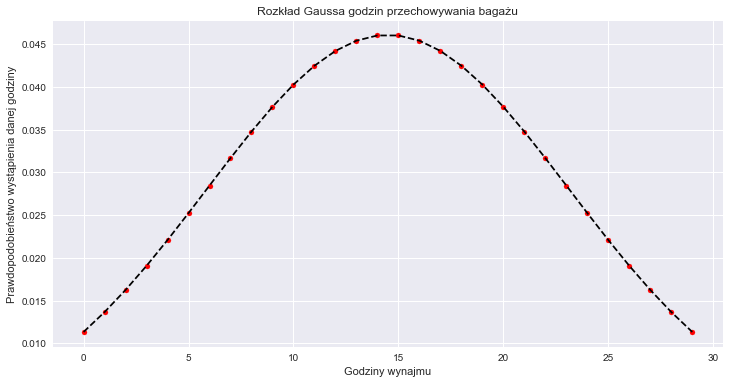
\includegraphics[ height=8cm]{godziny_gauss.png}
  \caption{Rozkład Gaussa}
  \label{figure_example}
\end{figure}

\subsection{Ilość klientów dziennie}
Dane zostaną wygenerowane przy użyciu rozkład gamma

\begin{figure}[H]
  \centering
  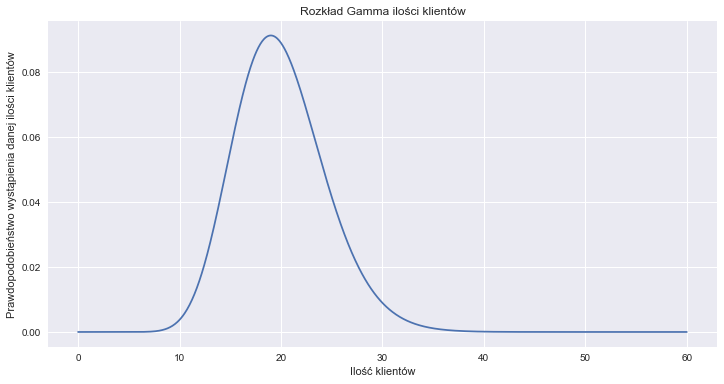
\includegraphics[ height=8cm]{gamma_klienci.png}
  \caption{Rozkład Gamma}
  
\end{figure}

\subsection{Rodzaj bagażu}
Dane zostaną wygenerowane przy użyciu rozkład jednostajnego

\begin{figure}[h]
  \centering
  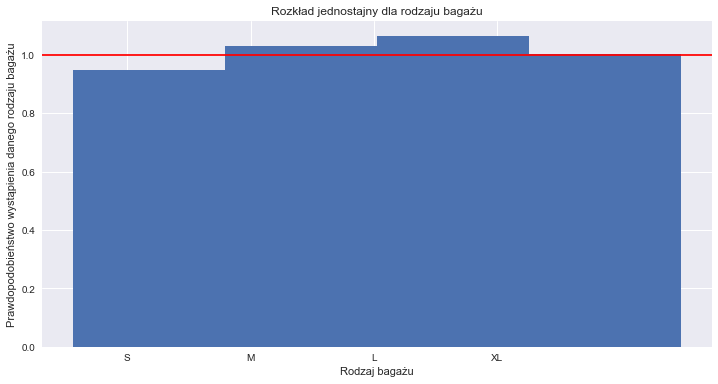
\includegraphics[ height=8cm]{baggage.png}
  \caption{Rozkład jednostajny}
  
\end{figure}

\section{Metody przypisania paczki do skrytki}
\subsection{Metoda oparta o maksymalizację zysków}
Metoda będzie kładła nacisk na jak największy zysk, który może wygenerować przedsiębiorstwo. Problem będzie badany za pomocą optymalizacyjnego algorytmu problemu plecakowego, dzięki któremu tak dobierzemy odpowiednią skrytkę do danego bagażu, aby zysk w $n$ dni był jak największy.

\subsection{Metoda losowa}
Będziemy losowo dobierać skrzykę do bagażu, zgodnie z ograniczeniami opisanymi w założeniach modelu matematycznego. W tej metodzie sprawdzimy jaki zysk będzie miało przedsiębiorstwo jeśli decyzja o przypisaniu paczki będzie losowa.
\section{Testy statystyczne}
\subsection{Sprawdzenie czy dane dot. ilości godzin pozostawienia bagażu w skrytce pochodzą z rozkładu jednostajnego }
Zostanie zastosowany test $\chi^2$ \\

\subsection{Sprawdzenie czy dane dot. ilości dziennej klientów pochodzą z rozkładu gamma }
Sprawdzimy za pomocą wykresu kwantyl-kwantyl (Q-Q plot), który przedstawi pozycję  kwantyli w wygenerowanych danych. Przez co będziemy mogli porównać, czy wykres zgadza się z wykresem dot. rozkładu gamma.
\subsection{Sprawdzenie czy dane dot. rodzaju bagażu pochodzą z rozkładu normalnego }
Zostanie zastosowany test Kołmogorowa-Smirnowa.
\section{Wnioski}

\end{document}